\documentclass{article}
\usepackage{tikz}

\begin{document}

\begin{figure}[h]
    \centering
    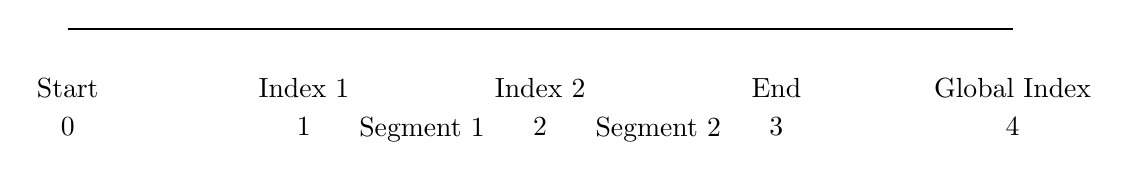
\begin{tikzpicture}[thick]
        % Draw the horizontal line
        \draw (0,0) -- (12,0);
        
        % Add nodes for labels and numbers
        \node at (0,-0.5) [below] {Start};
        \node at (3,-0.5) [below] {Index 1};
        \node at (6,-0.5) [below] {Index 2};
        \node at (9,-0.5) [below] {End};
        \node at (12,-0.5) [below] {Global Index};
        
        % Break the line into two segments
        \draw[dashed] (3,0) -- (6,0);
        \draw[dashed] (6,0) -- (9,0);
        
        % Add labels to the segments
        \node at (4.5,-1) [below] {Segment 1};
        \node at (7.5,-1) [below] {Segment 2};
        
        % Add numbers along the line
        \foreach \x/\y in {0/0, 3/1, 6/2, 9/3, 12/4} {
            \node at (\x,-1) [below] {\y};
        }
    \end{tikzpicture}
    \caption{Horizontal Line Divided into Two Segments}
    \label{fig:horizontal_line}
\end{figure}

\end{document}